\chapter{Grammatical Evolution}
\section{Introduction}
This chapter introduces the main elements of Grammatical Evolution~\cite{ieee2001}~\cite{ge_book}. It begins by providing an overview of grammars, in particular, focusing on the Backus Naur form used by GE. It also provides brief descriptions of derivation trees and parse trees, two important conceptual tools used to describe the application and structure of a grammar. The basic mechanism of GE is also introduced showing a step-by-step evolution of a solution using a simple grammar. Many of the terms associated with GE and referenced in the following chapters are also introduced here.



\section{Grammars}
\label{grammars}
Grammars provide a means of formally describing a language. Grammars consist of rules, which determine the linguistic structure of sentences in the language, terminals, which are the words or symbols of the language, and non-terminals, which expand into one or more terminals. In a \emph{context free grammar} (CFG) the syntax of a symbol, terminal or non-terminal is the same regardless of what other symbols surround it. Where there is a single non-terminal the grammar can be described as \emph{closed}~\cite{ripple}. 

Backus Naur Form (BNF), an example of which is shown in Figure~\ref{simple_grammar}, is a convenient descriptive notation for context free grammars is a notation for expressing the grammar of a language in the form of production rules. BNF consists of \emph{terminals}, which are items that can appear in the language, e.g. + - * etc. and \emph{non-terminals}, which can be expanded into one or more terminals and non-terminals.
A grammar can be represented by the tuple $<N,T,P,S>$ , where N is the set of non-terminals, T the set of terminals, P a set of production rules used to map elements of N to T. S a start symbol is a member of N.


\begin{figure}[tbp]
\begin{tabular}{p{12.8}}
\begin{verbatim}
N = {expr,op}
T = {+,-,/,*,X,(,)}
S = <expr>
P is a set of rules:
<expr>     :: == <var> | <expr><op><expr> | <pre-op>(<expr>)
                 | (<expr>) 
<var>      :: == X  	                                           
<op>       :: == + | - | * | /                            
<pre-op>   :: == sin | cos | tan | log        
\end{verbatim}
\end{tabular}
\caption{\label{simple_grammar}Example Grammar presented in Backus Naur Form.}
\end{figure}

\begin{figure}[tbp]
\centerline{\hbox{
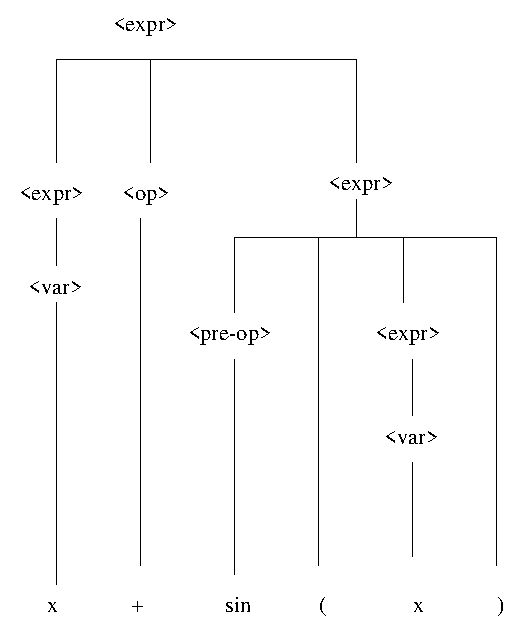
\psfig{file=Chapter2/graphs/derivation_tree.ps,width=3in}}}
\caption{Derivation Tree for the Expression $x + sin(x)$.}
\label{derivation_tree}
\end{figure}

\subsection{Derivation Trees}
A derivation tree is a way of showing graphically  the derivation of a sentence from a grammar. The generation of an expression in GE can be represented in this form. Figure~\ref{derivation_tree} shows a derivation tree for the expression $x + sin(x)$ using the simple grammar shown above. At the top of this tree we see the first derivation step in which the non-terminal $<expr>$ is replaced by $<expr><op><expr>$.  



\subsection{Parse Trees}
\label{parse_trees}
A parse tree concerns itself only with terminals. It assists the breakdown of the linguistic structure of the language. The parse tree for the expression $x + sin(x)$ is shown in Figure~\ref{parse_tree}.

\begin{figure}[tpb]
\centerline{\hbox{
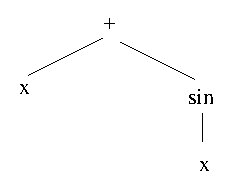
\psfig{file=Chapter2/graphs/parse_tree.ps,width=2in}}}
\caption{ Parse Tree for the Expression $x + sin(x)$.}
\label{parse_tree}
\end{figure}


\section{A Description of the Method}
\label{modulo}Grammatical Evolution (GE)~\cite{ieee2001}~\cite{ge_book} is an evolutionary algorithm that can evolve complete programs in an arbitrary language using a variable-length binary string. The binary string is decoded into a genome, which in turn is used to select production rules from a Backus Naur Form (BNF) grammar definition.  The system, illustrated in Figure~\ref{ge_fig1}, can use any search mechanism capable of generating a variable length sequence of integer codons. The codons, typically in the range 0 - 255, are used to select productions from the target grammar using the following function:
\small
\begin{displaymath}
\emph{Rule = (Codon value) MOD(Number of Rules for the current non-terminal)}
\end{displaymath}
\normalsize
A number of different codon values in the range 0 - 255 can cause selection of the same production rule. This occurs because the number of production rules associated with any non-terminal is generally small relative to the 256 expressible by a codon. This \label{sec:degeneracy} \emph{Genetic Code Degeneracy}~\cite{ieee2001} permits \emph{neutral mutation} which allows subtle changes in the search space without necessarily impacting the solution space (see Section~\ref{degeneracy}).

\begin{figure}[tbp]
\centerline{\hbox{
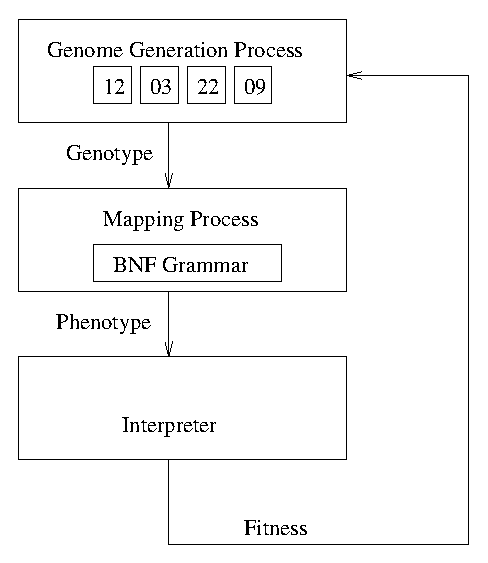
\psfig{file=Chapter2/graphs/ge_fig1.ps,width=3in}}}
\caption[Grammatical Evolution model.]{Grammatical Evolution, any metaheuristic capable of generating a variable length genome can be used with the system.}
\label{ge_fig1}
\end{figure}

Wrapping\label{sec:wrapping} is a technique employed by GE which allows the mapping process re-use codons from the genome. Once all codons in a genome have been used the process simply wraps to the start of the genome and continues the mapping process helping to improve the probability of a complete mapping of individuals onto programs.
 
The fitness associated with a solution is provided by evaluating the phenotype (i.e.,the program) using an interpreter for the target problem class. This fitness value is available to the generation mechanism to influence the future direction of the search strategy.
The following example illustrates the process of GE for the following simple expression: 


\begin{displaymath}
f(x) = sin(x) + x^2 + x
\end{displaymath}

A grammar, which can be used to derive this simple expression, is shown below.

\small
\label{sect:simple_grammar_bnf}\begin{verbatim}

<expr>   :: == <var> | <expr><op><expr> | <pre-op>(<expr>)
                     | (<expr>) 
<var>    :: == X  	                                           
<op>     :: == + | - | * | /                            
<pre-op> :: == sin | cos | tan | log        

\end{verbatim}
\normalsize

We present this grammar in tabular form in Figure~\ref{simple_grammar_table} and show the mapping process that occurs once the search engine has presented a codon to GE.

\begin{table}[h]
\begin{center}
\begin{tabular}{|l|l|l|l|l|l|}
\hline
\multicolumn{2}{|l|}{Non-Terminals}
&\multicolumn{4}{|l|}{Productions} \\
\hline
\multicolumn{2}{|l|}{ }
& 0 & 1 & 2 & 3 \\
\hline
1. & \verb|<expr>| & \verb|<var>| & \verb|<expr><op><expr>| & \verb|<pre-op>(<expr>| & \verb|(<expr>)| \\
2. & \verb|<var>| & X & & & \\
3. & \verb|<op>| & + & - & * & / \\
4. & \verb|<pre-op>| & sin & cos & tan & log \\
\hline
\end{tabular}
\caption{\label{simple_grammar_table}Simple grammar presented in table form.}
\end{center}
\end{table}



GE can use a depth first or a breadth first approach when mapping the codon string to an expression. The example shown in Table~\ref{bf_grammar_table1} and Table~\ref{bf_grammar_table2} illustrates the depth first approach which employs expansion of the left most non-terminal as the expression is created. Detailed commentary has been provided on the first nine derivation steps. The expanding non-terminal is shown in bold type through out Table~\ref{bf_grammar_table1} and Table~\ref{bf_grammar_table2} while the genome string used is shown in Figure~\ref{genome1}. Depth first expansion has been used in all of the trials reported in later sections.

\begin{figure}[!hbp]
\centerline{\hbox{

\psfig{file=Chapter2/graphs/genome1.xfig.ps,width=4in}}}
\caption{\label{genome1}Genome used in example of mapping process.}
\end{figure}


\begin{table}[!hbp]
\begin{center}
\begin{tabular}{|l|l|}
\hline
Step & Expression \\
\hline
0 & $ <expr>$ \\ 
  &     Start symbol. \\     
\hline
1 & $ ( \mathbf{<expr>} )$ \\ 
  &    11 mod 4 = 3, Production 3 from row 1 was chosen. \\
\hline
2 & $ ( \mathbf{<expr>} <op> <expr> )$ \\
  &    57 mod 4 = 1, Production 1 from row 1 was chosen. \\
\hline
3 & $ (( \mathbf{<expr>}) <op> <expr> )$  \\
  &    91 mod 4 = 3, Production 3 from row 1 was chosen. \\    
\hline
4 & $ ((\mathbf{<var>}) <op> <expr> )$ \\ 
  &   148 mod 4 = 0, Production 0 from row 1 was chosen. \\
\hline
5 & $ (( X ) \mathbf{<op>} <expr> )$  \\
  & There is only one choice for $<var>$ \\ 
  & so no codon was used for the transition to X. \\
\hline
6 & $ (( X ) * \mathbf{<expr>} )$ \\
  &  22 mod 4 = 2, Production 2 from row 4 was chosen. \\
\hline
7 & $ (( X ) * \mathbf{<expr>} <op> <expr> )$ \\
  &  129 mod 4 = 1, Production 1 from row 1 was chosen. \\ 
\hline
8 & $ (( X ) * \mathbf{<expr>} <op> <expr> <op> <expr> )$ \\
  & 53 mod 4 = 1, Production 1 from row 1 was chosen. \\
\hline
\hline
\end{tabular}
\caption{\label{bf_grammar_table1}Analysis of Depth First Mapping.}
\end{center}
\end{table}

\begin{table}[!hbp]
\begin{center}
\begin{tabular}{|l|l|}
\hline
Step & Expression \\
\hline
9 &  $ (( X ) * ( \mathbf{<expr>}) <op> <expr> <op> <expr>)$ \\ \hline
10 & $ (( X ) * (( \mathbf{<expr>})) <op> <expr> <op> <expr>)$ \\  \hline
11 & $ (( X ) * (( <var> )) \mathbf{<op>} <expr> <op> <expr>)$  \\ \hline
12 & $ (( X ) * (( X )) \mathbf{<op>} <expr> <op> <expr>)$  \\ \hline
13 & $ (( X ) * (( X )) + \mathbf{<expr>} <op> <expr>)$  \\ \hline
14 & $ (( X ) * (( X )) + \mathbf{<var>} <op> <expr>)$  \\ \hline
15 & $ (( X ) * (( X )) + X \mathbf{<op>} <expr>)$  \\ \hline
16 & $ (( X ) * (( X )) + X + \mathbf{<expr>})$  \\ \hline
17 & $ (( X ) * (( X )) + X + \mathbf{<pre-op>} (<expr>))$ \\ \hline
18 & $ (( X ) * (( X )) + X + Sin (\mathbf{<expr>}))$  \\ \hline
19 & $ (( X ) * (( X )) + X + Sin (\mathbf{<var>}))$  \\ \hline
20 & $ (( X ) * (( X )) + X + Sin (X))$  \\
\hline
\end{tabular}
\caption{\label{bf_grammar_table2}Analysis of Depth First Mapping (continued).}
\end{center}
\end{table}

\section{Expressed and Unexpressed Codons} 
A feature of GE is the ability to use only those codons which are required to effect a successful mapping. The genome string presented to GE could, for example, contain 30 codons, if only 15 of these are required to map a successful solution then the remaining 15 remain unexpressed. Though these codons are unexpressed they are not completely redundant, because the polymorphic nature of GE means that these codons could come in to play as that genome evolves through mutation or recombination.

\section{Genetic Code Degeneracy and neutral mutation}
\label{degeneracy} Genetic code degeneracy is a phenomenon that can be observed in the genetic code of biological organisms~\cite{elseth}. It occurs where there is redundancy in the coding required to specify aspects of the DNA. This redundancy can neutralise the effects of mutation in cases where the mutated bits are those that are redundant to the coding. Kimura's neutral theory of evolution  ~\cite{kimura} suggests that it is \emph{neutral mutations} that are responsible for the genetic diversity found in natural populations.
 
Genetic code degeneracy occurs in GE by virtue of the fact that even though a codon can represent 256 distinct integer values, many of these values represent the same production rule. For example using the \emph{MOD rule} with 4 productions would result in codon values 8, 4, 12 and 16 all selecting the same production 0. It is apparent from this that genomes with differing codon compositions can map to the same solution.
This property of GE, which permits \emph {neutral mutation} on redundant codings, allows subtle changes in the search space without necessarily impacting the solution space.



\section{Summary}
This chapter has introduced Grammatical Evolution, showing in detail how a variable length string of integer values can be used to derive an expression in any language given a suitable grammar. An introduction was provided to the subject of language grammars with particular focus on the Backus Naur Form. The concepts of genetic code degeneracy, neutral mutation, and expressed and unexpressed genes were also introduced. 












